\documentclass{beamer}
\usepackage[utf8]{inputenc}

\author[Sowmya Vajjala]{Instructor: Sowmya Vajjala}


\title[LING 120]{LING 120: Language and Computers}
\subtitle{Semester: FALL 2017}

\date{23 Aug 2017}

\institute{Iowa State University, USA}

%%%%%%%%%%%%%%%%%%%%%%%%%%%


\begin{document}

\begin{frame}\titlepage
\end{frame}

\begin{frame}
\frametitle{Class outline}
\begin{enumerate}
\item What is it about language that makes it difficult for computers? %10min
\item Encoding language on computers
\begin{itemize}
\item Writing systems %10min 
\item Storing different writing systems on computer %10min
\end{itemize}
\item Small group exercise (computer based)
\end{enumerate}
\end{frame}

\begin{frame}
\frametitle{Some language processing scenarios for computers}
\end{frame}

\begin{frame}
\frametitle{Computers and human language-1}
\framesubtitle{Google Home demo}
Girl: Okay Google, what's apples in Spanish?
\\ Google: (answers)
\\ ****** 
\\ Woman: Change my dinner reservation tonight, 7:30 to 8pm.
\\ Google: Your reservation for XXX is confirmed for 8pm. 
\\ source: \url{https://www.youtube.com/watch?v=2KpLHdAURGo}
\end{frame}


\begin{frame}
\frametitle{Computers and human language-2}
\framesubtitle{from 2011: Watson beats humans in Jeopardy}
\url{https://www.youtube.com/watch?v=WFR3lOm_xhE}
\end{frame}

\begin{frame}
\frametitle{Where do language and computers interact in real-world?}
\begin{enumerate}
\item Apple Siri and other such software that can understand and interpret human speech (okay, partially)
\item Google Translate and the likes
\item Search Engines
\item Question Answering (e.g., IBM Watson)
\item News recommendation - related articles features in News websites
\item Sentiment analysis of product reviews on Amazon, for example
\item Spam classification in Gmail, Yahoomail etc
\item Information extraction from text (e.g., identifying calendar entries automatically in gmail)
\item Dialog systems (having interactive conversations with users, to do flight bookings etc)
\item Spelling and grammar checkers
\end{enumerate}
... and many more. 
\end{frame}

\begin{frame}
\frametitle{Let us take a small text snippet}
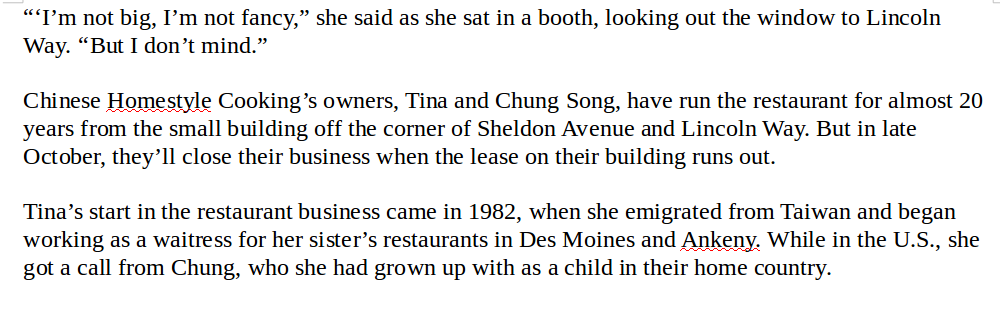
\includegraphics[width=0.9\textwidth]{Example.png}
\\ \footnotesize{Source: Ames Tribune (\url{http://goo.gl/zvx9Uw})}

\begin{enumerate}
\item When she says "I" in the first sentence, does she mean herself literally? \pause
\item What is she referring to? When will we know what is she referring to? \pause
\item Who is "She"? \pause
\item What is "home country" in the last sentence?  
\end{enumerate}
\end{frame}

\begin{frame}
\frametitle{More Questions}
\frametitle{Let us take a small text snippet -2}
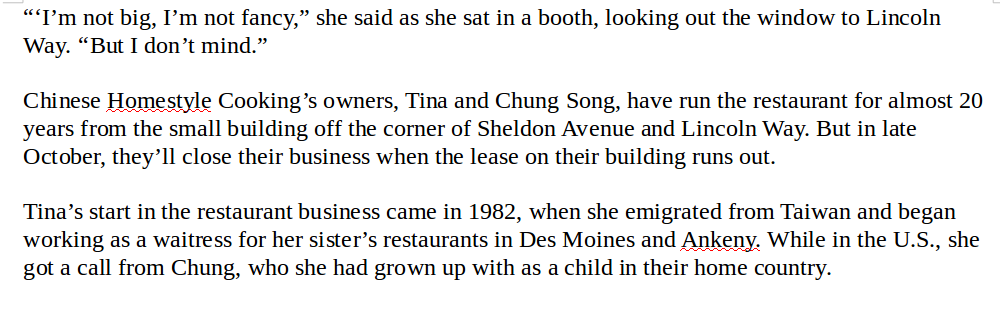
\includegraphics[width=0.9\textwidth]{Example.png}
\\ \footnotesize{Source: Ames Tribune \url{http://goo.gl/zvx9Uw}}
\begin{enumerate}
\item What is the main event of this text? \pause
\item What is "Chinese Homestyle Cooking" referring to? \pause
\item What is the relationship between "Chinese Homestyle cooking" and Tina? \pause
\item Is Lincoln Way something related to President Lincoln?
\end{enumerate}
\end{frame}

\begin{frame}
\frametitle{So ... }
\begin{itemize}
\item Each question I asked is a language processing problem for the computer which is not completey solved yet! \pause
\item ... and I only gave example of just one language (different languages may have different issues interms of processing) \pause
\item But before even getting in to that, how do we even represent language on a computer? What does a computer see when I type English or Greek or Chinese? \pause
\item How do I type non-English characters anyway??
\end{itemize}
\end{frame}

\begin{frame}
\frametitle{Encoding language on computers - Background}
\begin{itemize}
\item Computer stores any kind of information (including language) in bits and bytes (did you hear this before?) \pause
\item What is a bit? \pause (it is the short form of binary digit - 0 or 1)
\item What is a byte? \pause (a unit of information comprising of 8 bits)
\item How many different ways can we put 0s and 1s into 8 bit sequences? \pause $2^8$
\\ $\Rightarrow$ We can represent 256 different characters with 8 bits on a computer!
\end{itemize}
%Talk about ASCII here.
\end{frame}


\begin{frame}
\frametitle{ASCII - a 7 bit encoding}
\begin{itemize}
\item American Standard Code for Information Interchange (ASCII) is one of the early encoding systems for computers for storing English text.
\item It used only 7 bits to encode different characters.
\end{itemize}
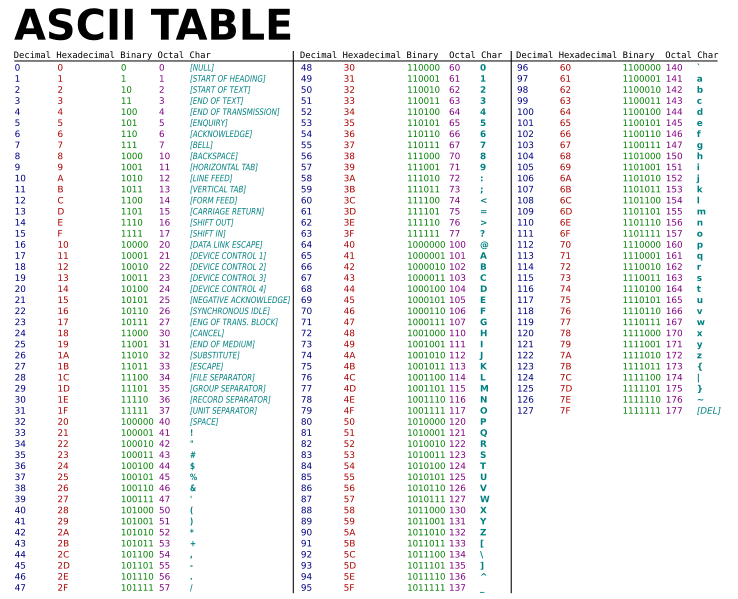
\includegraphics[width=0.6\textwidth]{ascii.png}
\\ image source: commons.wikimedia.org
\end{frame}

\begin{frame}
\frametitle{Writing Systems}
\begin{itemize}
\item So English is covered by ASCII
\item What should we do about several other languages written with different scripts?
\item My language (Telugu) has 56 basic characters in the alphabet, and some 20 other additional characters that attach to these. 
\item Russian alphabet has has around 40 characters.
\item There are several Indian language scripts like Telugu, having so many characters.
\item There are languages such as Chinese which have 100s of characters.
\end{itemize} \pause
... clearly ASCII cannot account for all these! What is the solution?
\end{frame}

\begin{frame}
\frametitle{Different encodings for different languages}
\begin{itemize}
\item Just extend the ASCII to 8 bits and use the remaining numbers (128-255) for adding new characters.
\item Several such encodings exist: ISO-8859-1 -adds additional characters for French, German Spanish; ISO-8859-8 for Hebrew etc. \pause
\item Problems with such an approach? \pause
\begin{enumerate}
\item Two different encodings can have same number for different characters
\item One character can get different numbers in two different encodings
\end{enumerate}
\item So what?: \pause
\begin{enumerate}
\item If the encoding information is not provided in the webpage, a browser needs to guess. Guessing is difficult with those two problems.
\item Each time I want to see a new language, I need a new encoding, install and setup process to work with it!
\end{enumerate}
\end{itemize}
\end{frame}

\begin{frame}
\frametitle{Solution: Unicode}
\begin{itemize}
\item Aim: a single representation to represent all characters in all existing writing systems (\url{unicode.org}). \pause
\item How does it do this?: it uses a 32 bit representation instead of 8 bit!
\item So, how many characters can it represent? \pause $2^{32} = 4,294,967,296$! 
\item Do we really need so many?
\item What are the advantages and disadvantages of this 32 bit representation?
\end{itemize}
\end{frame}

\begin{frame}
\frametitle{UTF-8, UTF-16, UTF-32}
\begin{itemize}
\item Unicode has three representations (UTF- Unicode Transformation Format) - the numbers represent the number of bits needed to represent a character in that representation. \pause
\item How can $2^{32}$ combinations be represented with $2^{16}$ or $2^{8}$ combinations itself?? \pause
\item The idea is to use variable number of bytes to represent a character (instead of 1 byte all the time or 4 bytes all the time)
\item How to do that?: Use the left most bits as "flags" to tell the computer about number of bytes used per character. i.e., if the starting bit is 1, it means there is only character. Starting two bits are 11 means - you should expect two bytes per character, and so on. \pause
\item Good thing about this is: ASCII is already UTF-8, you don't have to change anything.
\end{itemize}
\end{frame}

\begin{frame}
\frametitle{UTF-8 Details}
\begin{itemize}
\item First byte tells you how many bytes to expect. e.g., if you see something like 11110xxx, you know you should expect this character to be of four bytes.
\item Second byte on, everything starts with 10 to indicate that it is not the first byte in that sequence. 
\item Let us take the example of the Greek character $\alpha$. In Unicode, its value is 945, which in binary is 11 10110001. What is this with 32 bits? \pause
\item 00000000 00000000 00000011 10110001
\item How can we represent this number with UTF-8? \pause
\item \textbf{11}001110 \textbf{10}110001
\end{itemize}
\end{frame}

\begin{frame}
\frametitle{A small exercise}
open \url{zh.wikipedia.org} in Firefox browser, and find out what the encoding of that page is. Usually, you will also see a host of other encodings - what other options do you see?. What happens if you choose a different encoding instead of the one shown? Post the answer in today's forum to get attendance for today.
\end{frame}

\begin{frame}
\frametitle{Next Class}
\begin{itemize}
\item Topic: Encoding spoken language
\item Assignment 1 description 
\item ToDo: Read chapter 1
\end{itemize}
\end{frame}

%exercise on wednesday show this: see a webpage, what encoding is it showing? what happens if we change the encoding?
%page 30, prob 7: exercise for attendance on friday. 

\end{document}

% With some examples, establish that we know certain senses from context and world knowledge, but how can computer know?
-15min

%Fundamental issue before even talking about such things: What is a computer looking at when we type letters? Why do we need to bother? - because there are several writing systems.

%Writing systems of the world:
-15 min

%How do we encode written language on computers?
bits, bytes, binary, hexadecimal, big endian, little endian,
decimals to binary
-10 min

%Exercise: 10 min (What? Something involving language and computers here)


%Day 4: I can talk about typing in different languages etc. 
